\begin{figure*}[t]
  \centering
  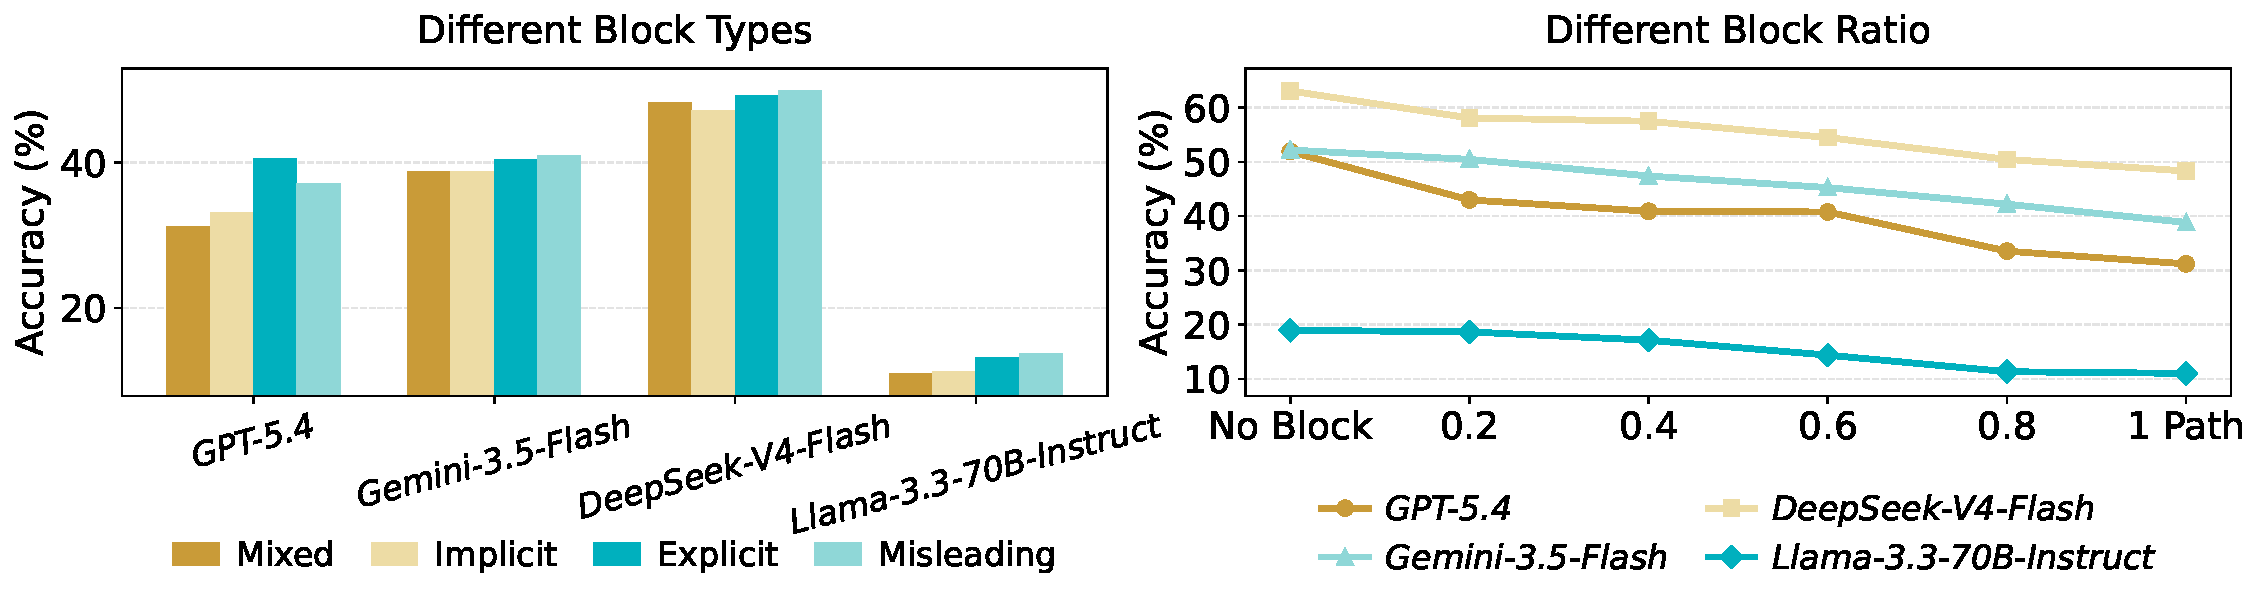
\includegraphics[width=1\linewidth]{Figures/noise_combined_pdf.pdf}
  \vspace{-0.25in}
  \caption{Accuracy under retrieval-time blocking. \textit{\textbf{Left}}: performance across different block types when only one feasible solution path remains, including mixed blockers (\textit{Mixed}), implicit failures (\textit{Implicit}), explicit failures (\textit{Explicit}), and semantic distractions (\textit{Misleading}). \textit{\textbf{Right}}: performance as blocking becomes stronger, ordered from no-block to block ratios of 0.2, 0.4, 0.6, and 0.8, with “1 Path” leaving only a single feasible path.}
  \label{fig:noise_combined}
  \vspace{-0.1in}
\end{figure*}